\begin{frame}
    \begin{center}
    \begin{tabular}{ccc}
        \visible<1->{
\includegraphics[width=0.3\linewidth]{figures/platypus.pdf}} &
        \visible<2->{ \Huge VS} &
        \visible<3->{
\includegraphics[width=0.3\linewidth]{figures/wa-logo-stacked2-large.png}}
    \end{tabular}
    \end{center}
\end{frame}

\subsection{Future work}

\begin{frame}
    \frametitle{Better database}

    Not answered by \alert{Wikidata}:
    \begin{itemize}
      \item ``How fast is the TGV?''
      \item ``How wide is a tennis court?''
    \end{itemize}

    \medbreak

    $\rightarrow$ Improve Wikidata?

    $\rightarrow$ Use another database?
\end{frame}

\begin{frame}
    \frametitle{Better question parsing}

    Not parsed correctly:
    \begin{itemize}
      \item ``What is the date of birth of Isaac Newton?''
      \item ``In which band does Bono sing?''
    \end{itemize}

    \medbreak

    $\rightarrow$ Train the Stanford \alert{CoreNLP} library?

    $\rightarrow$ Improve the algorithm of the Grammatical module?

    $\rightarrow$ Better datasets for the ML modules?
\end{frame}

\begin{frame}
    \frametitle{New modules}
\begin{figure}
 \begin{tikzpicture}
  \node (0) at (-3,2) {\textcolor{mLightBrown}{cooking recipes}};
  \node (0) at (1,1) {\textcolor{mDarkBrown}{HAL}};
  \node (0) at (5,2.5) {\textcolor{mMediumBrown}{meteo}};
  \node (0) at (3,2) {\textcolor{mDarkTeal}{train timetable}};
  \node (0) at (0,0) {\textcolor{mMediumBrown}{programming language interpreter}};
  \node (0) at (-4,-1) {\textcolor{mMediumBrown}{cinema}};
  \node (0) at (0,-2) {\textcolor{mDarkTeal}{music}};
  \node (0) at (4,-1) {\textcolor{mDarkTeal}{literature}};
  \node (0) at (-3,-2) {\textcolor{mDarkBrown}{OEIS}};
  \node (0) at (2,-2.5) {\textcolor{mLightBrown}{translation}};
  \node (0) at (-2,-3) {\textcolor{mMediumBrown}{sport statistics and predictions}};
  \end{tikzpicture}
\end{figure}
\end{frame}

\begin{frame}
    \frametitle{Other ideas...}

    \begin{itemize}
        \item Other languages support (French...)
        \item Improve user experience
        \item Advertise \alert{Platypus}
    \end{itemize}
\end{frame}

\subsection{Conclusion}

\begin{frame}
    \frametitle{Some facts} % to update just before the presentation
    \alert{23 repositories \& 2313 commits}

    \begin{tabular}{lll}
        6 & PHP & Wikidata libraries and module\\
        12 & Python & Other modules, core, and libraries\\
        1 & C++ & ML-Reformulation\\
        1 & Shell & Deployment scripts\\
        1 & \LaTeX & This presentation and the report\\
        1 & Markdown & The specification\\
        1 & HTML/CSS/Javascript & The Web User Interface\\
    \end{tabular}

    \alert{26k lines} of code (13k in PHP, 10k in Python)

    \alert{4.3k lines} of Latex \& \alert{2.9k lines} of Markdown

    \alert{4} accepted pull requests to libraries we use (corenlp-python, aspell-python, python-datautil)
\end{frame}

\begin{frame}
    \frametitle{The PPP?}

    \begin{itemize}
        \item A powerful question answering framework
        \item Innovative NLP algorithms
        \item A demo, \alert{Platypus}, with general knowledge and math
    \end{itemize}
\end{frame}


\newlength{\logosize}
\setlength{\logosize}{12pt}
\begin{frame}
    \frametitle{Questions?}
    
    \begin{columns}
    \begin{column}{0.55\textwidth}
        \alert{\url{http://projetpp.github.io/}}\vspace{5pt}
        \begin{tabular}{ll}
            
\includegraphics[width=\logosize]{Twitter_logo_blue.png} & \href{https://twitter.com/ProjetPP}{https://twitter.com/ProjetPP}\\
            
\includegraphics[width=\logosize]{GitHub-Mark-32px.png} &  \href{https://github.com/ProjetPP}{https://github.com/ProjetPP}\\
            
\includegraphics[width=\logosize]{ic_email_black_18dp.png} & \href{mailto:ppp@pony.ovh}{ppp@pony.ovh}\\
        \end{tabular}
    \end{column}
    \begin{column}{0.5\textwidth}
        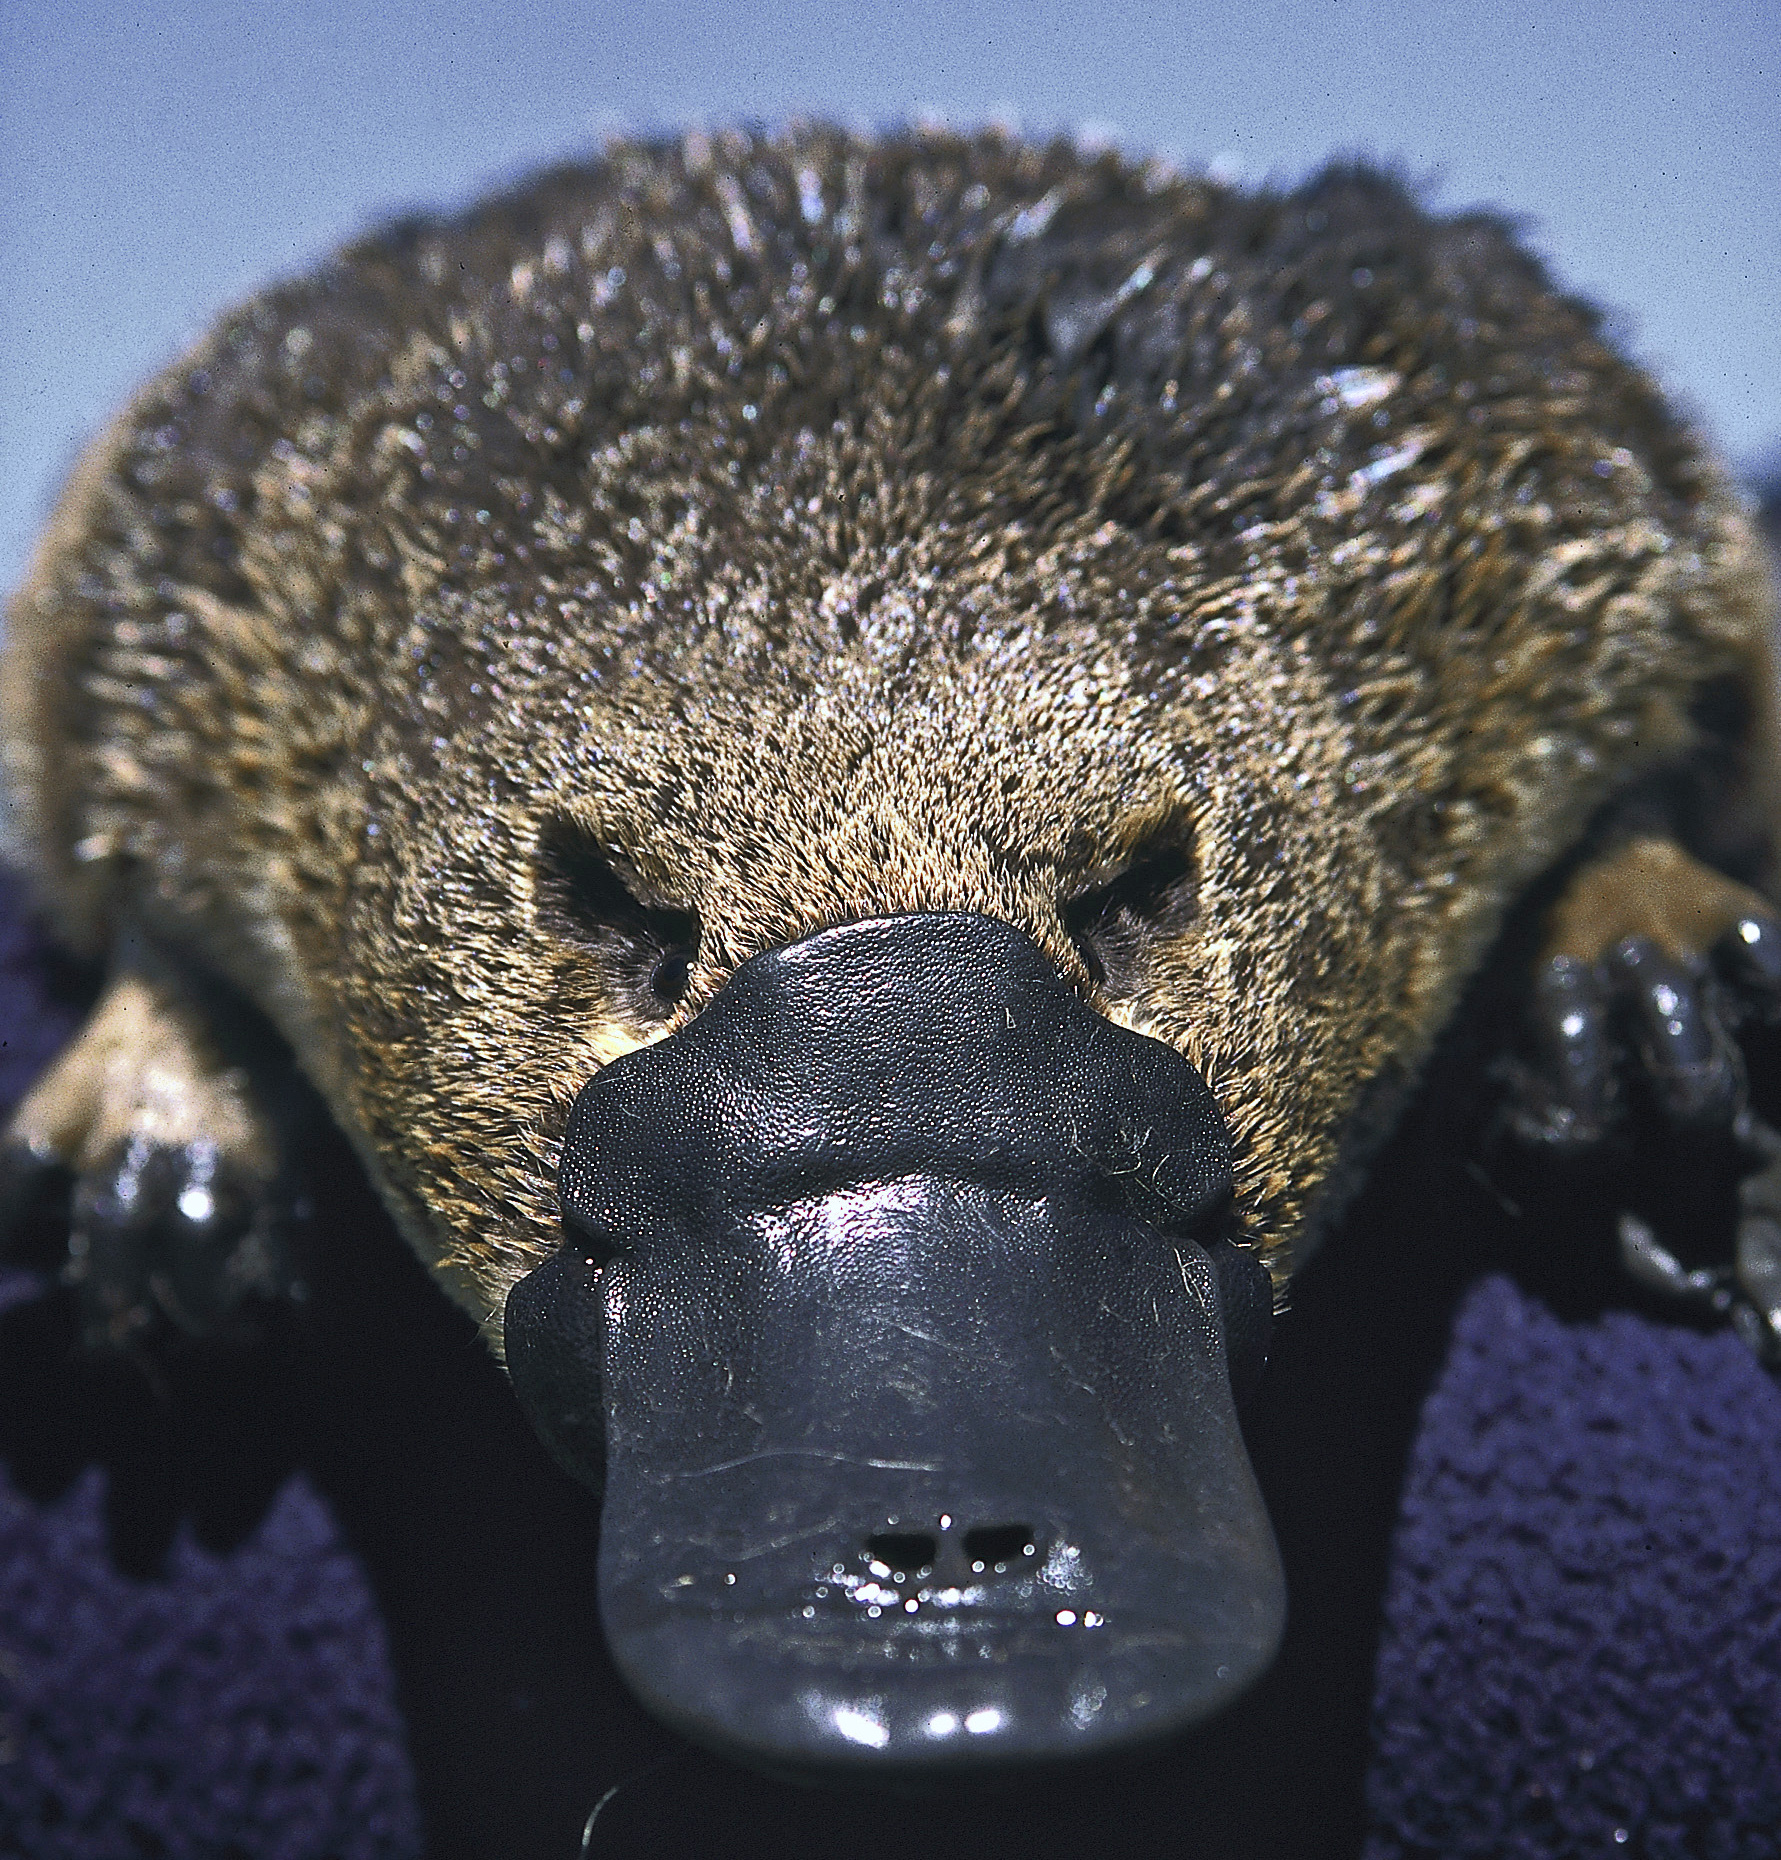
\includegraphics[width=\linewidth]{figures/Ornithorhynchus.jpg}
    \end{column}
    \end{columns}
\end{frame}

\begin{frame}
    \tikzset{
        workpackage/.style={
               node distance = 0.5cm,
               },
    }
    \frametitle{WorkPackages}
    \begin{figure}
        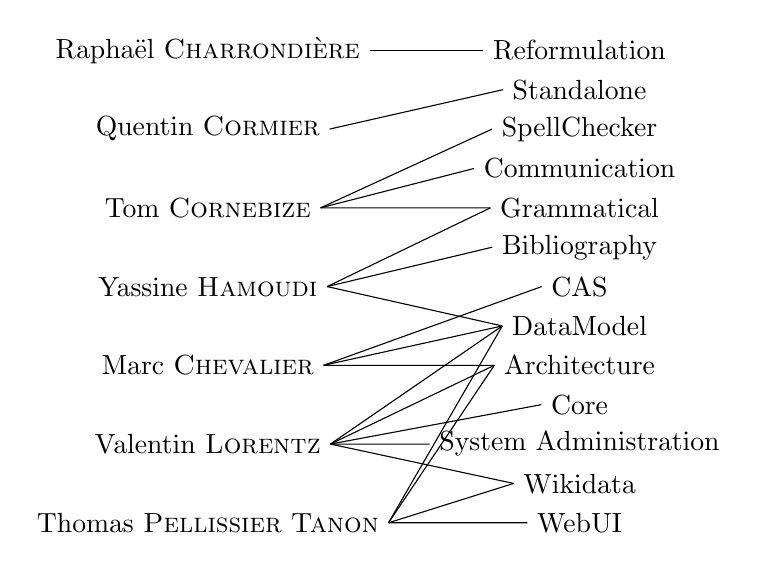
\begin{tikzpicture}
            % PPP members
            \node (rc)                  {Raphaël \textsc{Charrondière}};
            \node (qc)  [below of = rc] {Quentin \textsc{Cormier}};
            \node (tc)  [below of = qc] {Tom \textsc{Cornebize}};
            \node (yh)  [below of = tc] {Yassine \textsc{Hamoudi}};
            \node (mc)  [below of = yh] {Marc \textsc{Chevalier}};
            \node (vl)  [below of = mc] {Valentin \textsc{Lorentz}};
            \node (tpt) [below of = vl] {Thomas \textsc{Pellissier} \textsc{Tanon}};

            % PPP WorkPackages
            \node (reformulation)   [workpackage, right of = rc, right=3cm]  {Reformulation};
            \node (standalone)      [workpackage, below of = reformulation]  {Standalone};
            \node (spellchecker)    [workpackage, below of = standalone]     {SpellChecker};
            \node (communication)   [workpackage, below of = spellchecker]   {Communication};
            \node (grammatical)     [workpackage, below of = communication]  {Grammatical};
            \node (bibliography)    [workpackage, below of = grammatical]    {Bibliography};
            \node (cas)             [workpackage, below of = bibliography]   {CAS};
            \node (datamodel)       [workpackage, below of = cas]            {DataModel};
            \node (architecture)    [workpackage, below of = datamodel]      {Architecture};
            \node (core)            [workpackage, below of = architecture]   {Core};
            \node (sysadmin)        [workpackage, below of = core]           {System Administration};
            \node (wikidata)        [workpackage, below of = sysadmin]       {Wikidata};
            \node (webui)           [workpackage, below of = wikidata]       {WebUI};

            % Edges
            \path (reformulation.west)   edge (rc.east)
                  (standalone.west)      edge (qc.east)
                  (spellchecker.west)    edge (tc.east)
                  (communication.west)   edge (tc.east)
                  (grammatical.west)     edge (tc.east)
                  (grammatical.west)     edge (yh.east)
                  (bibliography.west)    edge (yh.east)
                  (datamodel.west)       edge (yh.east)
                  (datamodel.west)       edge (mc.east)
                  (datamodel.west)       edge (vl.east)
                  (datamodel.west)       edge (tpt.east)
                  (architecture.west)    edge (mc.east)
                  (architecture.west)    edge (vl.east)
                  (architecture.west)    edge (tpt.east)
                  (cas.west)             edge (mc.east)
                  (core.west)            edge (vl.east)
                  (sysadmin.west)        edge (vl.east)
                  (wikidata.west)        edge (vl.east)
                  (wikidata.west)        edge (tpt.east)
                  (webui.west)           edge (tpt.east);
        \end{tikzpicture}
    \end{figure}
\end{frame}

\begin{frame}
    \begin{center}
        \Huge Demo time!
    \end{center}
\end{frame}

\begin{frame}[plain]
    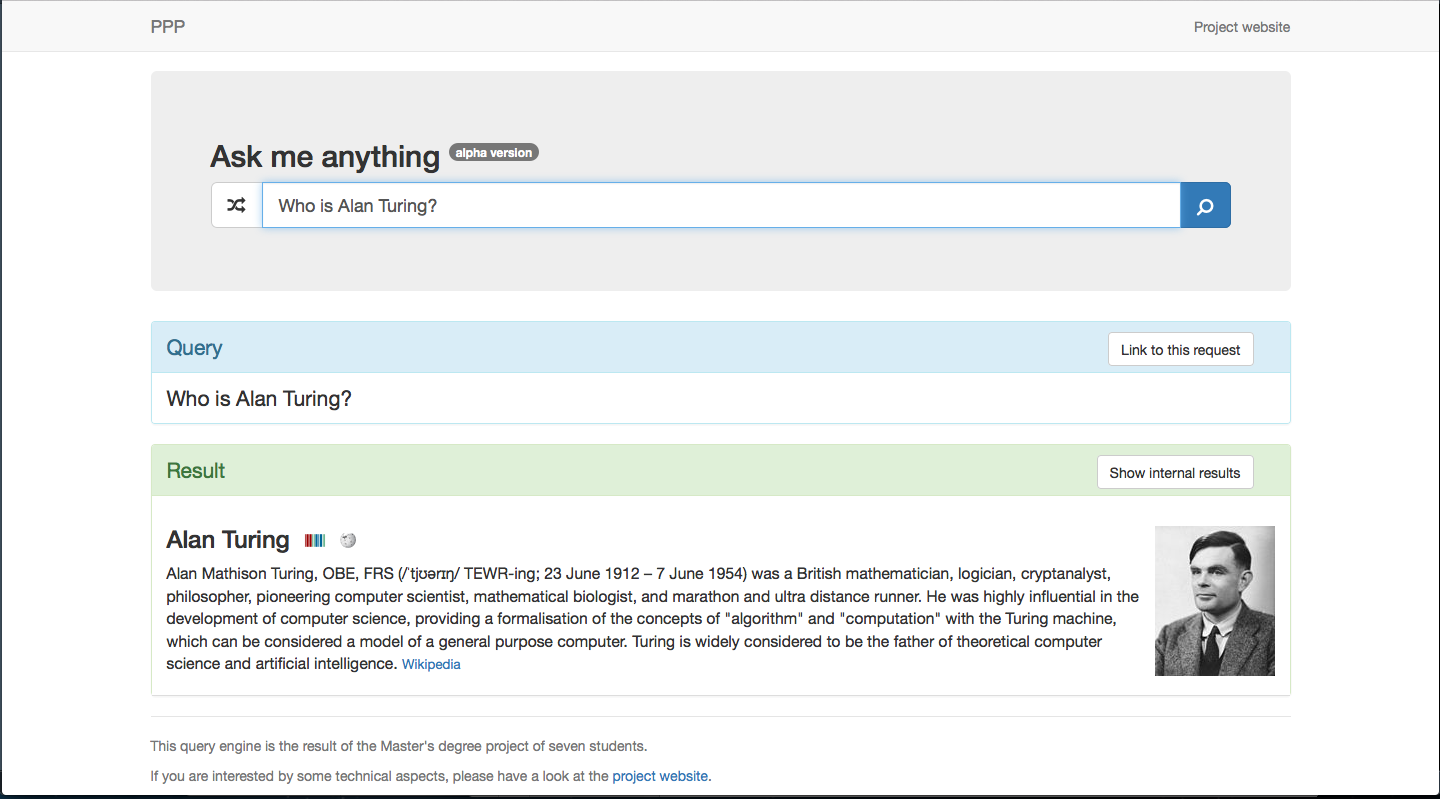
\includegraphics[width=\linewidth]{figures/demo-whoIsAlanTuring.png}
\end{frame}

\begin{frame}[plain]
    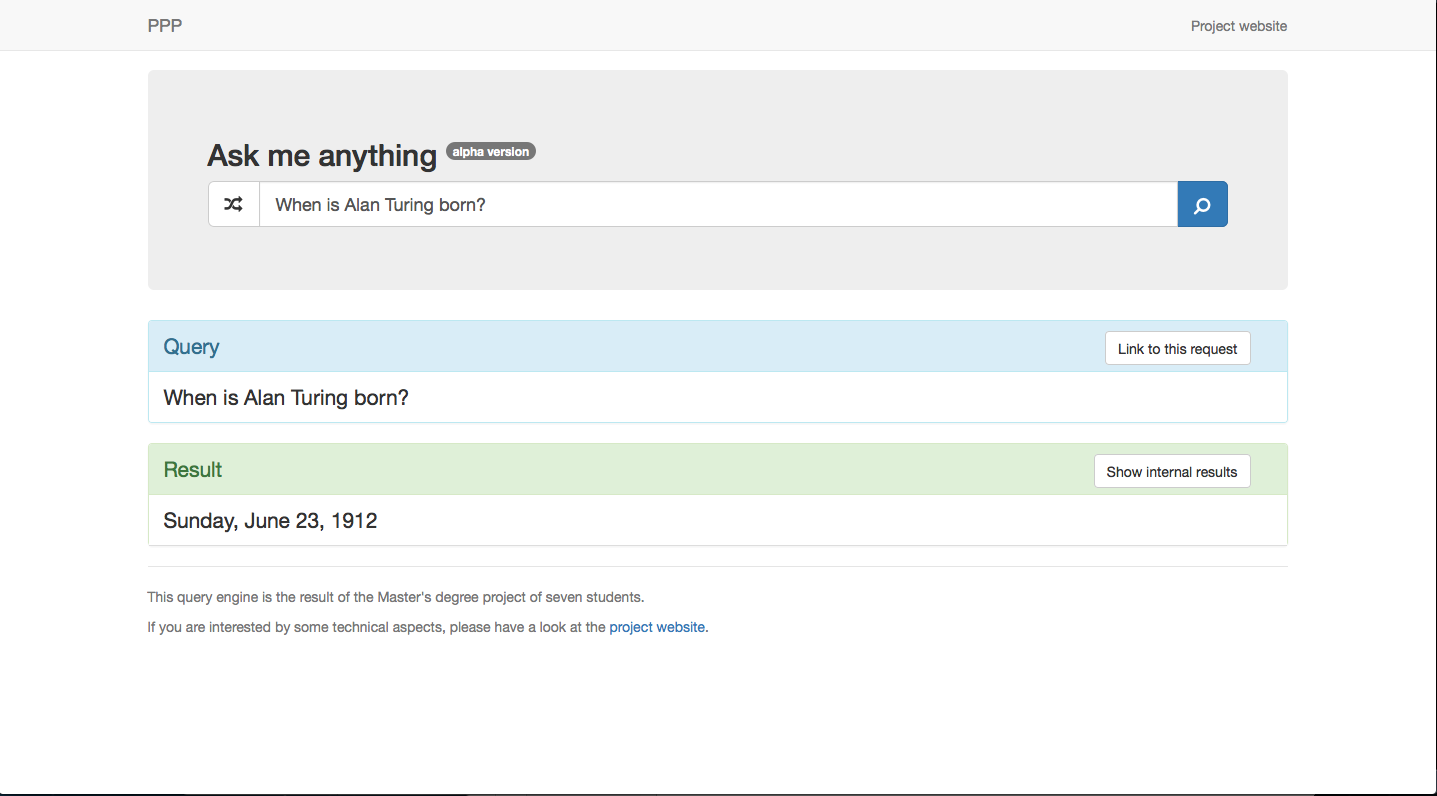
\includegraphics[width=\linewidth]{figures/demo-whenIsAlanTuringBorn.png}
\end{frame}

\begin{frame}[plain]
    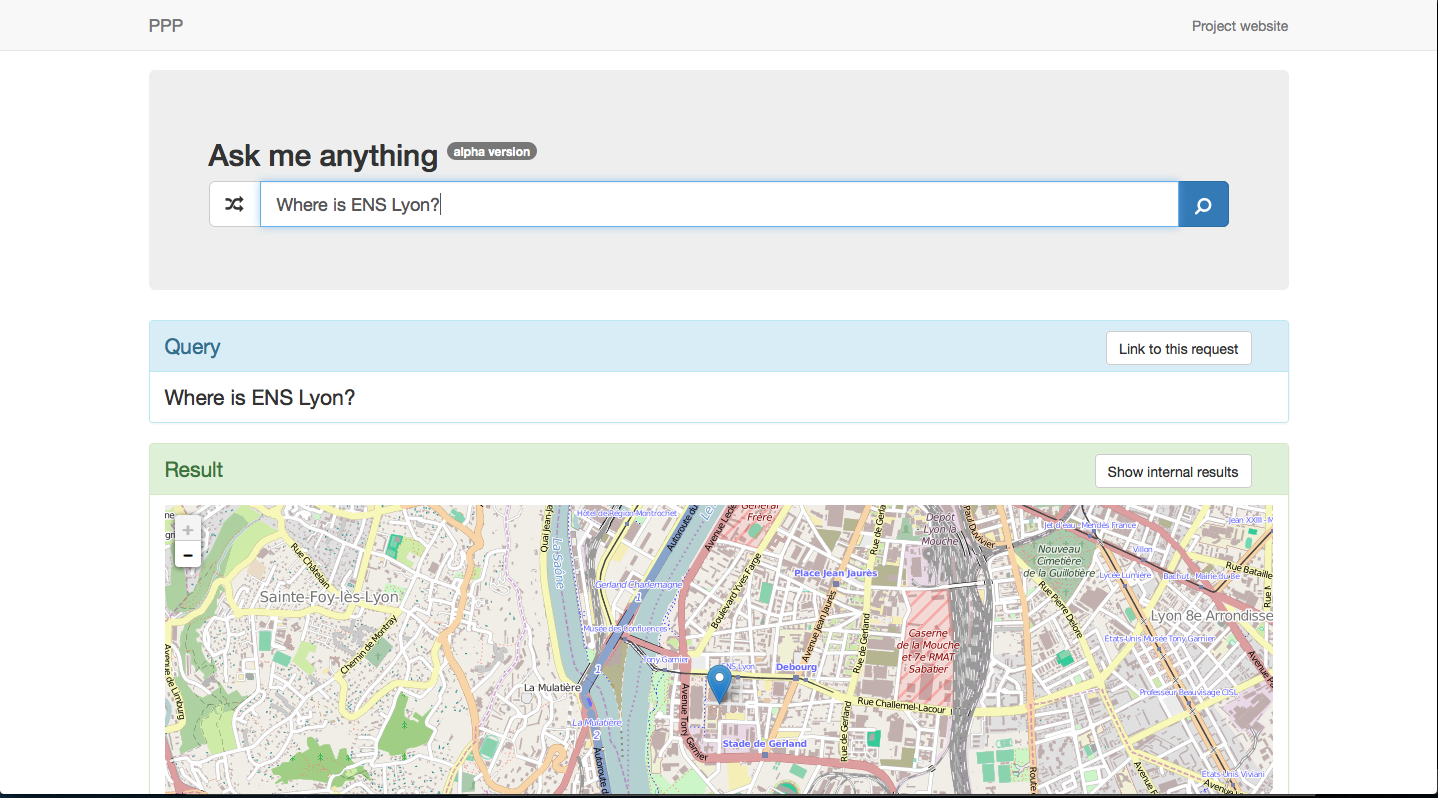
\includegraphics[width=\linewidth]{figures/demo-whereIsEnsLyon.png}
\end{frame}

\begin{frame}
    \begin{center}
    \begin{tabular}{ccc}
        \visible<1->{
\includegraphics[width=0.3\linewidth]{figures/platypus.pdf}} &
        \visible<2->{ \Huge VS} &
        \visible<3->{
\includegraphics[width=0.3\linewidth]{figures/wa-logo-stacked2-large.png}}
    \end{tabular}
    \end{center}
\end{frame}

\begin{frame}
    \frametitle{Nested question}

Who is the wife of the president of the United States?
    \begin{tabular}{ll}
        \alert{WolframAlpha} & Barack Obama\\
        \alert{Platypus} & Michelle Obama\\
    \end{tabular}

    \medbreak

    \onslide<2->{
        What are the birth dates of the daughters of the wife of the president of the United States?
        \begin{tabular}{ll}
            \alert{WolframAlpha} & Barack Obama\\
            \alert{Platypus} & Saturday, July 4, 1998 \& Sunday, June 10, 2001\\
        \end{tabular}
    }
\end{frame}

\begin{frame}[fragile]
    \frametitle{Conjunction}

Who is the actor of Inception and Titanic?
    \begin{tabular}{ll}
        \alert{WolframAlpha} & all the actors of the two movies\\
        \alert{Platypus} & Leonardo DiCaprio\\
    \end{tabular}
\end{frame}

\subsection{Spell checker}

\begin{frame}[fragile]
    \frametitle{Spell Checker}
    Based on \alert{GNU Aspell}.

    \medbreak

    \onslide<2->{
        What are the langajes of Soth Afryka?

        $\rightarrow$

        What are the languages of South Africa?
    }

    \medbreak

    \onslide<3->{\alert{120 lines of code} $\Rightarrow$ quickness of module creation.}
\end{frame}
